\documentclass[12pt,letterpaper]{article}
\usepackage[utf8]{inputenc}
\usepackage{amsmath}
\usepackage{amsfonts}
\usepackage{amssymb}
\usepackage{amsthm}
\usepackage{graphicx}
\usepackage{tabularx}
\usepackage[left=2cm,right=2cm,top=2cm,bottom=2cm]{geometry}
\usepackage{multicol}
\usepackage{lastpage}
\usepackage{fancyhdr}
\usepackage{multirow,array}
\usepackage{newtxtext,newtxmath}
\usepackage{lastpage}
\usepackage{enumitem}
\newcolumntype{Y}{>{\centering\arraybackslash}X}
\pagestyle{fancy}
\fancyhf{}
\lhead{\textsc{BHCC Mat-181}}
\chead{\textsc{Answers}}
\rhead{\textsc{HW Exercises 1.48-1.64}}
\rfoot{Page \thepage ~of \pageref{LastPage}}
\setenumerate[1]{label={\bf 1.\theenumi: }}
\setenumerate[2]{label={\bf (\theenumii): }}


\begin{document}
\begin{enumerate}
\setcounter{enumi}{47}

\item We first determine that IQR $ = 82.5-72.5 = 10$. From there we can check for outliers. The longest whisker length is $1.5\times 10 = 15$. 

The upper whisker could extend as far as $82.5+15 = 97.5$, which is higher than the maximum score. So, we won't have any outliers above the boxplot, and the upper whisker will extend to 94.

The lower whisker could extend as low as $72.5-15 = 57.5$. There is one score lower than this, so that score is a potential outlier (marked by a dot on the boxplot). The lower whisker won't reach the minimum score; instead, it will reach the second lowest score: 66.

\begin{center}
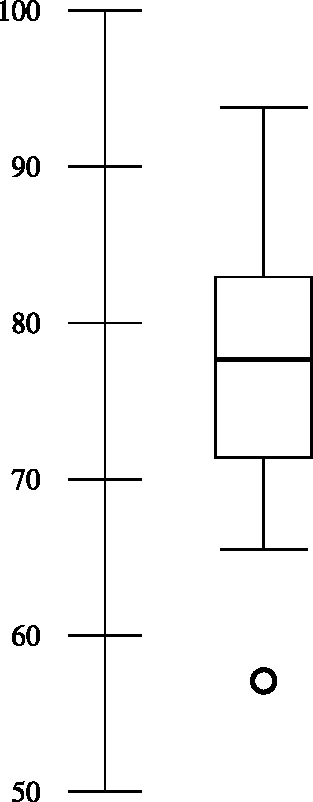
\includegraphics[scale=0.7]{figures/boxplot.pdf} 
\end{center}



\item \begin{enumerate}\item To estimate $Q_1$, we determine about how far along the horizontal axis we must move before reaching 25\% of the area. Because we have a relative frequency histogram, all of the bars stacked on top of each other would have a height of 1.

Because 37\% of countries have between 0 and 10 deaths, we know $Q_1$ is between 0 and 10. We are not exactly sure, but we might estimate that $Q_1 \approx 7$. 

The histogram shows 37\% of countries have between 0 and 10 deaths per 1000 births. Also, 23\% of countries have between 10 and 20 deaths per 1000 births. That means 60\% of countries have between 0 and 20 deaths per 1000 births. Somewhere between a death rate of 10 and 20 we reached the median. Median $\approx 15$.

If we add the first three bars we get $0.37+0.23+0.1 = 0.7$, still not 0.75. If we add the first four bars we get $0.37+0.23+0.1+0.05 = 0.75$, so it seems that $Q_3 \approx 40$.

\item The mean is larger than the median because of the rightward skew.
\end{enumerate}


\item \begin{enumerate}
\item Unimodal, symmetric, matches Plot 2.
\item Uniform, matches Plot 3.
\item Unimodal, right skew, matches plot 1.
\end{enumerate}

\item 
First, it is helpful to estimate the heights of the bars.
\begin{center}
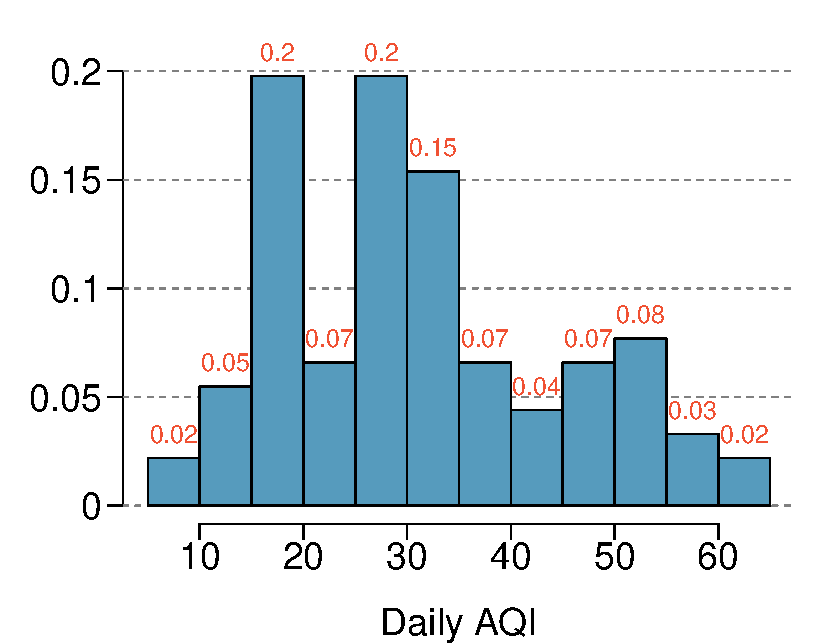
\includegraphics[scale=1]{figures/air_quality_durham_rel_freq_hist_soln}
\end{center}
\begin{enumerate}
\item The median is between 30 and 35, let's say 32.
\item This distribution is a bit skew right, so I'd say the mean is probably a bit higher than the median.
\item $Q_1 \approx 18$. $Q_3 \approx 38$. IQR $\approx 20$.
\item With my approximations, the lowest possible non-outlier AQI would be $18-1.5\times 20$, which is less than 0. The highest possible non-outlier would be $38+1.5\times 20 = 68$, which is higher than any of the AQIs. So it seems there are no unusually high or low AQIs (because in the histogram the lowest possible is 5 and highest possible is 65).
\end{enumerate}

\item It is helpful to start by labelling the frequencies. We also know the total should be 400.
\begin{center}
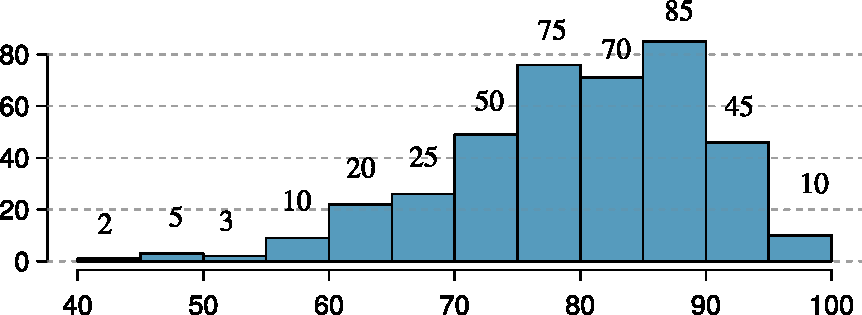
\includegraphics[scale=1]{figures/estimate_mean_median_simple_sol}
\end{center}
We can either tally from the left or the right, but either way we get to 200 observations between scores of 80 and 85. We can estimate a median of about 52.

\item The histogram shows the bimodal characteristic, and bin frequencies. The boxplot shows the median, quartiles, and possible outliers. 

\item \begin{enumerate}
\item The histogram shows the bimodal characteristic, and bin frequencies. The boxplot shows the median, quartiles, and possible outliers. 
\item The winning times for men tend to cluster at a significantly shorter time than winning times for women. The peak between 2 and 2.2 is due to fast men. The peak between 2.4 and 2.6 is due to fast women.
\item Both distributions seem skewed right, with possible outliers on the higher end. The IQR for men is smaller than the IQR for women. The men have a lower median than the women.
\item The time series show that over time both genders have gotten faster, but now seem to have leveled off.
\end{enumerate}

\item \begin{enumerate} \item The number of pets per household would probably have a right skew. Thus, it would be better to use median and IQR.
\item The distance to work is probably right skewed as there is a lower boundary of 0 and a few people probably travel very very far. Again, median and IQR are better. (However Exercise 1.63 makes it look pretty symmetric...)
\item Heights are probably nearly symmetric. In this case, mean and standard deviation work well.
\end{enumerate}

\item \begin{enumerate} \item These housing prices sound skew right. Skewed distributions should use median and IQR.
\item These housing prices sound symmetric. We can use mean and standard deviation.
\item The number of drinks is probably skew right, so we use median and IQR.
\item These salaries sound skew right, so we use median and IQR.
\end{enumerate}

\item It does not sound symmetric because the standard deviation is almost as large as the mean and it is impossible to watch negative hours of television. We expect this distribution to be skewed right.

\item There is a boundary at 100, and the mean is only one standard deviation below the boundary, so we can be pretty sure this distribution is skewed left.

\item The mean (190) is higher than the median (100), so the distribution is skewed right.

\item \begin{enumerate}
\item symmetric, the numerator $\bar{x}$ equals the denominator.
\item skew left, the median is larger than the mean.
\item skew right, the mean is larger than the median.
\end{enumerate}

\item \begin{enumerate}
\item The median is a better indicator. The median is more robust than the mean.
\item The IQR is better than standard deviation. The IQR is more robust.
\end{enumerate}

\item This measure is not robust to outliers. In fact, it is almost entirely determined by the outliers.

\item \begin{enumerate}
\item This distribution does not appear skewed. It seems symmetric. A log transformation does not seem very appropriate.
\item The areas with high commute times seem scattered about, maybe around large cities.
\end{enumerate}

\item \begin{enumerate}
\item The distribution is skewed right, so a log transformation might help us see more aspects of the distribution.
\item The map shows where the prevalence of hispanic people is high or low. The histogram gives a better summary of median, quartiles, and IQR.
\item Both visualizations are helpful for different situations.
\end{enumerate}

\end{enumerate}
\end{document}
